\begin{wrapfigure}{r}{0.25\textwidth} % 'r' for right positioning, 0.25 width
    \centering
    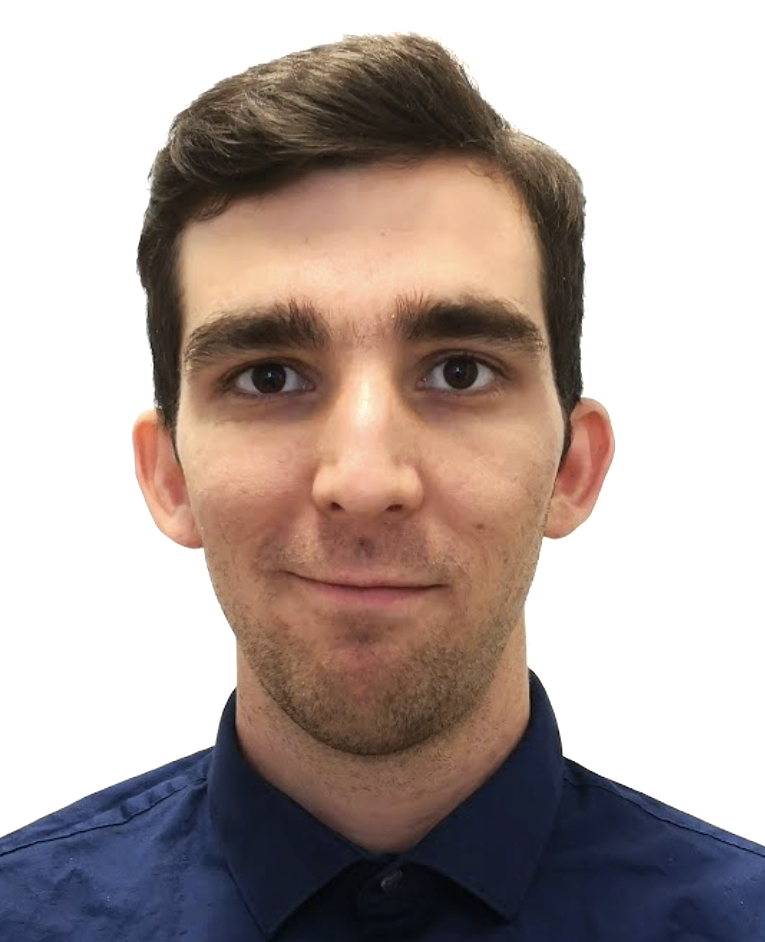
\includegraphics[width=0.24\textwidth]{src/avatar.png}
\end{wrapfigure}

{\noindent\huge\bfseries Mátyás Budavári}\\[0.5ex]
\small{Software Developer Team Lead}\\[1ex]


\noindent
\begin{tabular}{ll}
    LinkedIn: & \myurl{https://www.linkedin.com/in/budavariam/}{budavariam}\\
    Email:    & \myurl{mailto:\mymail{budavariam}}{\mymail{budavariam}}\\
    GitHub:   & \myurl{https://github.com/budavariam}{budavariam}\\
    Website:  & \myurl{https://budavariam.github.io}{budavariam.github.io}
\end{tabular}\\[2ex]

\noindent
I believe that learning is a lifelong process. \textbf{Software engineering} today is an ever-changing industry.
I like to keep track of its changes, and I deliberately \textbf{strive to be better} at what I do.
In my spare time, I like to \textbf{expand my knowledge} besides the technologies we use at work and write \textbf{blog posts} about them.

  